Hiring effectively is one of the key challenges faced by any organization.
There are two possibly conflicting optimization issues that a hiring committee faces when considering a candidate: 
(i) the value added to the organization in terms of the candidate's raw skills and competencies, and 
(ii) how well the candidate can collaborate with the existing members of the organization.
The first consideration depends on the complementarity between the candidate's skills and the tasks that the organization aims to complete. 
This is called \textit{coverage} in the team formation literature.
The second consideration is commonly known as the \textit{communication cost}.

In their seminal paper, Lappas et al. \cite{lappas2009finding} first introduced the problem of \textit{team formation}, where they modelled team in the form of a graph.
They proposed two graph distance-based measures of communication cost, namely the diameter and minimum spanning tree of the graph. 
They showed that the team formation problem is NP-complete for both types of communication costs. 
Subsequent works \cite{sozio2010community, kargar2011discovering, anagnostopoulos2010power, rangapuram2013towards} explored more realistic formulations of the team  formation problem. They study different cost functions and objectives that model the real world requirements more closely.
In \cite{bhowmik2014submodularity}, a submodular variant of the team formation problem is proposed, enabling an approximation guarantee for a simulated annealing algorithm.

Our work distinguishes itself by studying the problem of team formation from a organization's point of view. The major challeneges that an organizational setting provide are as follows. In a typical organization we already have a set of people that are part of the organization. The team formation decision needs to consider this existing set while making the choice. Moreover, the exact set of tasks is not known beforehand. The tasks vary depending on the progress the organization makes in different fronts. However, the organization does need to make decisions regarding the employees, such as whom to hire or fire based on those unforeseen tasks. In \cite{anagnostopoulos2012online}, authors assume that tasks arrive in an online manner. Thus once an assignment is made, it cannot be revoked later. In our problem formulation, we assume that tasks are drawn from a distribution. Therefore the tasks comes with a probability associated with them, which was not studied in \cite{anagnostopoulos2012online}. Thirdly, presence of organization opens up several new objectives that are not studied in typical team formation before. Since our tasks are probabilistic, we optimize these objectives under their expected values. 

To understand this better, refer to Figure \ref{fig:hpo}. Our problem has four inputs: an existing organization, a pool of candidates, a task distribution and the objective that we want to maximize. We consider four specific objectives in this work, namely \textit{hiring}, \textit{stupid hiring}, \textit{assassination} and \textit{firing}. 
 
\begin{figure}
\centering
\begin{small}
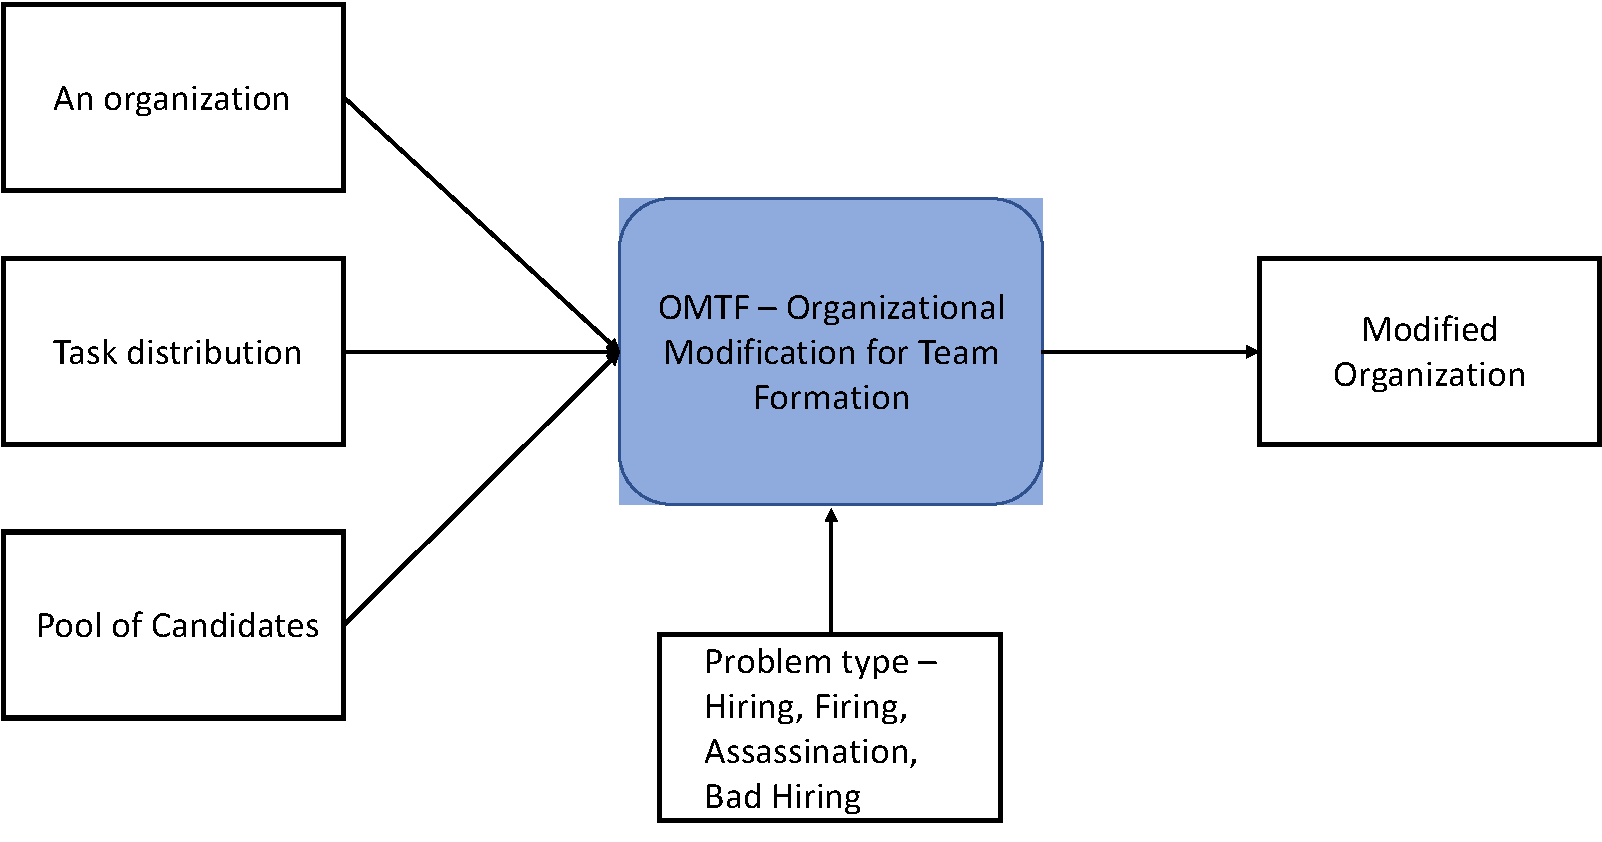
\includegraphics[width=.25\textwidth]{figs/pdf/illustration.pdf}
\caption{Hiring problem overview}
\label{fig:hpo}
\end{small}
\end{figure} 

In this paper, we show that the hiring problem is NP-hard. 
However, we provide two realistic communication and coverage functions such that both are submodular.
When both these functions are submodular, we can design a greedy approximation \cite{bai2016algorithms} that preserves a $1 - \frac{1}{e}$ - approximation.
Thus, to summarize, our contributions are the following:

\begin{enumerate}
\item We formulate the novel \textit{hiring problem}, which draws its inspiration from the team formation literature.

\item We show that the problem is NP-hard. 
However, under certain communication and coverage functions, efficient approximation algorithms can be designed for the problem.

\item By leveraging the work of \cite{bai2016algorithms}, we design a greedy algorithm that preserves a $1 - \frac{1}{e}$ approximation ratio.

\item Through extensive experiments on real world datasets, we empirically show the superiority of our approach over existing baselines. 

\end{enumerate}